\documentclass[border=2pt]{standalone}

% Drawing
\usepackage{tikz}
\usepackage{pgfplots}
\pgfplotsset{compat=1.18}

% Tikz Library
\usetikzlibrary{calc}

% Middle Line Label
\newcommand{\midlabelline}[3]{
   \node (midlabel) at ($ (#1)!.5!(#2) $) {\scriptsize#3};
   \draw[latex-] (#1) --  (midlabel);
   \draw[-latex] (midlabel) -- (#2);
}

% Define Color
\definecolor{chromeyellow}{rgb}{1.0, 0.65, 0.0}

\begin{document}
	
	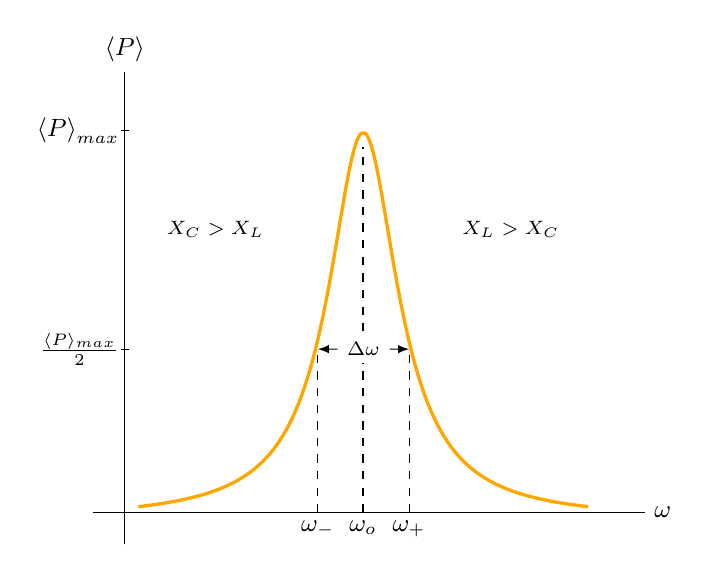
\begin{tikzpicture}
		% Grid
%		\draw[help lines] (0,0) grid (8,8);
		
		% Axis
		\draw (0,0.4) -- ++(7,0) node [right] {\small$\omega$};
		\draw (0.4,0) -- ++(0,6) node [above] {\small$\langle P \rangle$};
		
		% Plot
		\begin{axis}[
			xtick=\empty,
			ytick=\empty,
			axis line style={draw=none},
			]
			%
			\addplot[chromeyellow, samples=300, very thick] {50/(2+ (1.5*x - 1/(1000*x))^2)};
		\end{axis}
		
		% Text Labels
		%% y-Axis
		\draw (0.35,5.25) -- ++(0.1,0) node [left] {\small${\langle P \rangle}_{max}$};
		\draw (0.35,2.475) -- ++(0.1,0) node [left] {\small$\frac{\langle P \rangle_{max}}{2}$};
		%% delta omega
		\midlabelline{2.85,2.475}{4.01,2.475}{$\Delta\omega$}
		%% x-Axis
		\draw [dashed] (3.424,0.4) -- ++(0,1.9) node [pos=-0.1] {\small$\omega_o$};
		\draw [dashed] (3.424,2.7) -- ++(0,2.338);
		\draw [dashed] (2.85,0.4) -- ++(0,2.1) node [pos=-0.1] {\small$\omega_-$};
		\draw [dashed] (4.01,0.4) -- ++(0,2.1) node [pos=-0.1] {\small$\omega_+$};
		
		% Nodes
		\node at (5.3,4) {\scriptsize$X_L>X_C$};
		\node at (1.55,4) {\scriptsize$X_C>X_L$};
	\end{tikzpicture}
	
\end{document}